\section{Analysis}

As detailed in the literature review, branch coverage is the percentage of branches from conditional statements that have been executed. So for an \verb|if| statement, if it only ever evaluates to \verb|true| then the branch coverage at that vertex is 50\%. This becomes a problem when you have code such as in Figure \ref{lst:branchingExample}. If the \verb|if| statement always evaluates to true during testing, statement coverage will show as being over 99\%. However, if it ever evaluates to false then \verb|someObject| won't be initialised, and an exception will be thrown later on if somewhere else \verb|someObject| is referenced.

\begin{figure}
\centering
\begin{minipage}{.4\textwidth}
  \centering
  \lstinputlisting[language=EOL]{code/branch_example.java}
  %\caption{Some sample pseudocode}
\end{minipage}%
\begin{minipage}{.5\textwidth}
  \centering
  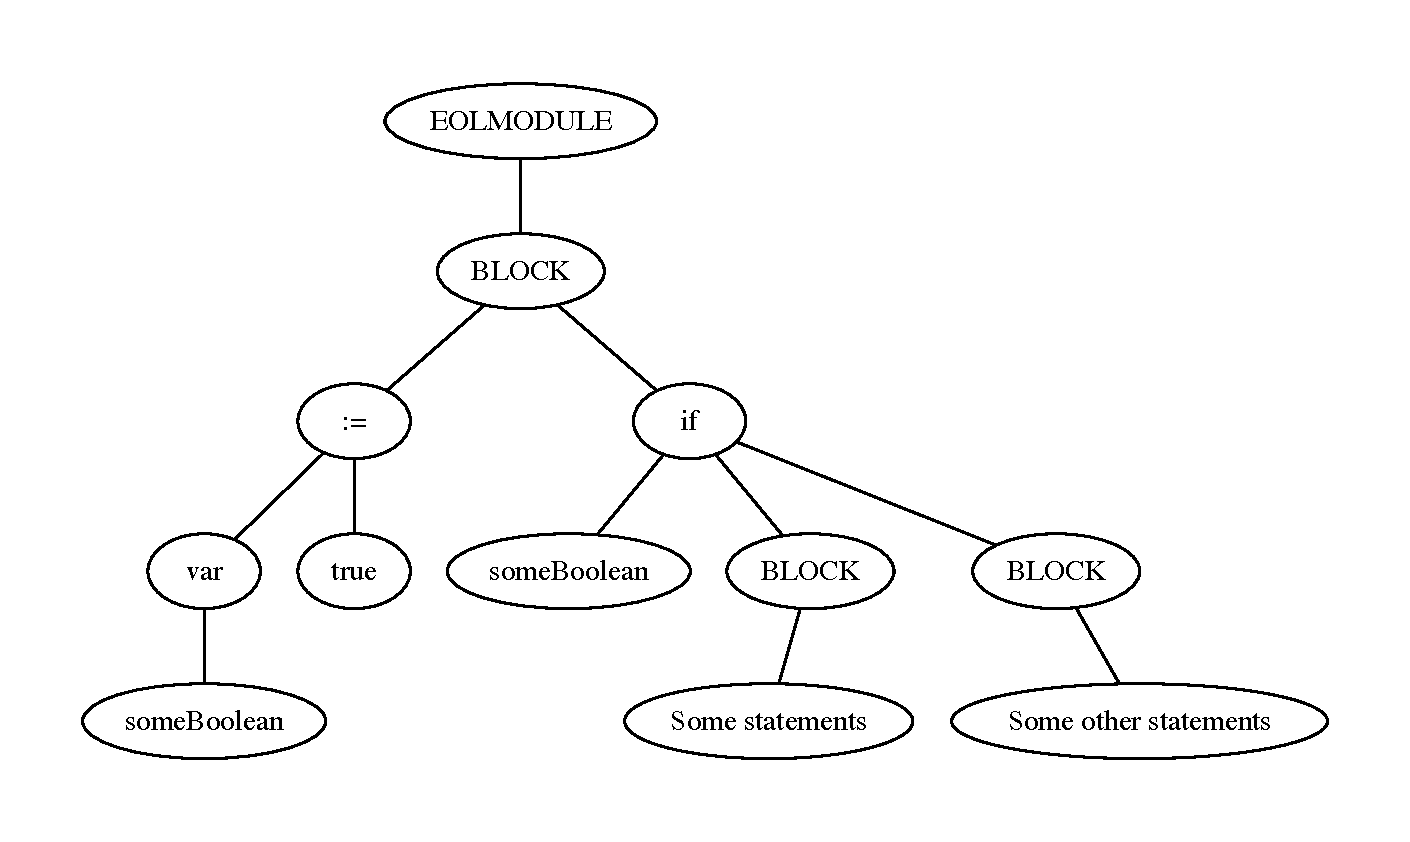
\includegraphics[scale=0.4]{figures/branchSampleAST.pdf}
  %\caption{The AST of the program in Figure \ref{lst:branchingExample}}
\end{minipage}
\caption{On the left is some sample pseudocode, and on the right is the AST for the sample pseudocode}
  \label{lst:branchingExample}
\end{figure}

Branch coverage can counter this by looking at how many of the possible paths after all conditional statements have been executed. So in the code in Figure \ref{lst:branchingExample}, only 50\% of possible paths from that \verb|if| statement have been executed, and so the branch coverage is 50\%.

By looking at the AST (Figure \ref{lst:branchingExample}) of the sample code, it would appear that by counting the number of blocks below the \verb|if| vertex, we could determine how many branches in the code there are, and after execution we could see how many of those branches have been executed.

Unfortunately this approach is not perfect. The blocks only appear when curly braces are used. If just a single statement is placed under the \verb|if| statement, then the block is skipped and just a vertex for the single statement appears. So this means that the code is now more complex than it was previously thought to be. Furthermore, \verb|if| statements can have children that never need to be executed (because they just contain information about the conditional), and so my algorithm would need to include details of this. If these were the only drawbacks then I would still choose this approach. However, this kind of caveat occurs for many conditional statements, and so the code that would be produced would be rather unwieldy and difficult to maintain.

The approach that I have chosen to take is actually quite difficult to justify. I suggest that the AST be converted to a Control Flow Graph (CFG), at which point the branches from each vertex will be clear. A record will be made on which edges between vertices have been executed, and the total number of edges will be counted. The edges that have not been recorded will map to the branches that were not taken. The reason that this is difficult to justify is that an extensive search has not come up with any explicit instructions on how to go about generating a control flow graph from an abstract syntax tree. \citet{grune2000modern} very briefly discuss the process of `threading' an AST to produce a CFG, but only state that there must be a subroutine that deals with each statement. Likewise, a set of lecture slides by \citet{compilersIntro} provide some brief details on a high level algorithm, but nowhere enough to implement it from scratch.

Some forward thinking means that the conversion from AST to CFG will be necessary when performing the path coverage because of the formula detailed in the literature review's path coverage section to calculate cyclomatic complexity, and so this effort will solve two problems, and will have a quicker overall development time. Designing this algorithm and detailing it will be one of the large contributions of this project because of the lack of other detailed literature about the AST to CFG conversion process.

Before beginning development, a list was made of the statements that need to be included. This was done by going through the Epsilon book \citep{epsilonBook} which is a complete source of EOL syntax, but also as well by going through the EuGENia source (the software used in the case study in Chapter \ref{chap:evaluation}) to see which statements are actually used in real EOL code. The list was then ordered loosely in priority based on the number of uses within the EuGENia source. The list as as follows:

\begin{enumerate}[nolistsep]
\item block
\item if
\item if .. else
\item for
\item while
\item switch
	\begin{enumerate}
	\item case
	\item default
	\item continue
	\end{enumerate}
\item operation
\item return
\item break
\item breakAll
\item continue
\end{enumerate}

For each of the identified statements, I will individually analyse how they can be converted from an AST to a CFG. For each statement a sample AST will be shown, as well as the desired CFG.

\subsection{Start and End}
As discussed in the literature review, a CFG starts with a START vertex, and ends with an END vertex. In all the examples below of a CFG, these vertices are present. Each example represents a small subsection of an EOL program. When viewing the examples, the START vertex could be imagined to be where any part of a larger program joins up to the example CFG, and similarly the END vertex can be imagined to be the continue point of the program, where the statements following the example would join up to.

\subsection{The Block}
A block is not actually a statement, but refers to a block of statements. Within a block can be any other set of statements, including other blocks. The contents of a block are often contained within \{ \} (curly braces or brackets), but not always (see the case statement).

The block is not conditional in any way. When represented in the AST, it can have any number of children, which are executed in order of first child (left-most) to last child (right-most). When a block is encountered in the AST by the conversion algorithm, it should simply be a case of joining the block vertex to the last statement that was encountered, and also joining it to the block's first child.

The code in Figure \ref{fig:block} is a whole EOL program. The whole program is inside a block statement, as can be seen by the AST in the same figure. There are two statements in the block, and in the AST each statement is represented as a child. In the CFG, each of the children are represented sequentially, so the first child is represented after the block, and then the second child after the first child.

The block could be left out of the CFG, as arguably it does not provide any more information about control flow. However it is valid syntax for a block to exist as a pair of brackets with no statements in, and so not including the block statement could cause problems in this case. For the rest of this analysis, the block statement may be used to represent any subset of vertices that does not add to the analysis. The input to the block vertex will represent input to the first vertex of the subset, and the output from the block will represent the output from any possible exit vertices from the subset.

\begin{figure}
\centering
\begin{minipage}{.3\textwidth}
  \centering
  \lstinputlisting[language=EOL]{code/statements/block.java}
  %\caption{}
  %\label{lst:blockStatement}
\end{minipage}%
\begin{minipage}{.3\textwidth}
  \centering
  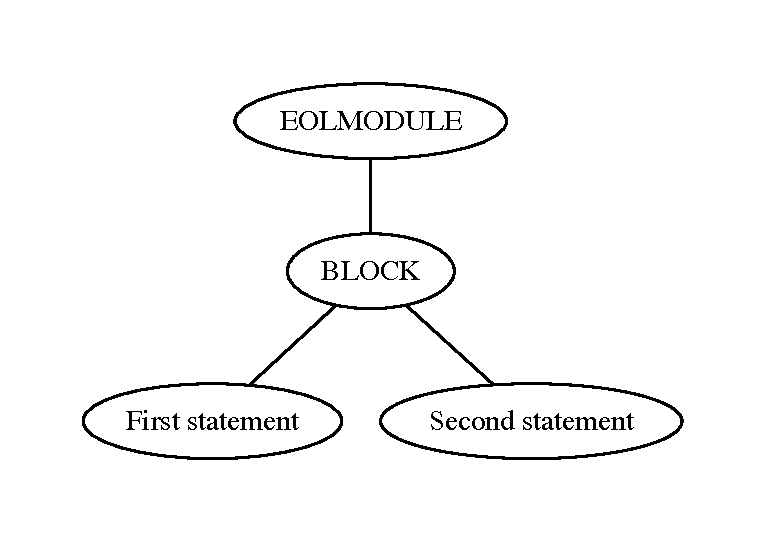
\includegraphics[width=\linewidth]{figures/statements/block_AST.pdf}
   % \caption{}
  %\label{fig:blockAST}
\end{minipage}
\begin{minipage}{.3\textwidth}
  \centering
  \includedot[scale=0.3]{figures/statements/block_CFG}
   % \caption{}
  %\label{fig:blockCFG}
\end{minipage}
\caption{From left to right: The block's code, AST and desired CFG}
\label{fig:block}
\end{figure}

\subsection{The if statement}

The if statement is going to be treated as a separate statement to the if .. else statement, because when it comes to designing and implementing the algorithm, different code will be required for each.

The \verb|if| statement evaluates its predicate, and if the predicate evaluates to true then it executes the code in the brackets that follow it, or if there are no brackets, it executes the statement that directly follows it. While the outcome of execution is the same (when there is only one statement executed following an \verb|if| statement that evaluates to true), the use of brackets following the if statement changes the structure of the AST in a way that must be considered during the conversion. Figure \ref{fig:if} shows the \verb|if| statement that uses brackets, and Figure \ref{fig:ifnoparen} shows the statement that does not use brackets.

When the brackets are used, if the \verb|if| predicate evaluates to false then the statement that immediately follows the block must be the next statement to be executed. This will be the sibling of the if statement in the AST. If the if statement evaluates to true, then once it has finished executing the block it must move on to the next statement after the block, which again will be the next sibling of the if statement in the AST. This of course is assuming that a statement within either of the blocks does not divert program flow away from the next statement. A simple example would be to imagine that the contents of the block shown in Figure \ref{fig:if} are modified to include a \verb|return| statement. This is not uncommon in a program, and so must be considered. In this case the the final statement will not be executed, because return will end the current program (or sub-routine).

When no brackets are used, the same rules almost apply. Except that rather than looking for the next statement after the block, it will be the second statement in the statements that follow the \verb|if| statement. This will still be represented in the AST as the next sibling of the if statement.

Another consideration must be made about program flow. Within the predicate of the if statement, any number of subroutines can exist. It could be viewed as another block of code, and this is why it appears as the first child of the if statement in the AST. For the purpose of control flow, this will be ignored. Any code within the predicate will not modify the flow of the program in this operation, and even then it will only evaluate to either true or false.

\begin{figure}
\centering
\begin{minipage}{.3\textwidth}
  \centering
  \lstinputlisting[language=EOL]{code/statements/if.java}
  %\caption{}
  %\label{lst:blockStatement}
\end{minipage}%
\begin{minipage}{.3\textwidth}
  \centering
  \includedot[width=\linewidth]{figures/statements/if_AST}
   % \caption{}
  %\label{fig:blockAST}
\end{minipage}
\begin{minipage}{.3\textwidth}
  \centering
  \includedot[scale=0.3]{figures/statements/if_CFG}
   % \caption{}
  %\label{fig:blockCFG}
\end{minipage}
\caption{From left to right: The if statement with brackets' code, AST and desired CFG}
\label{fig:if}
\end{figure}

\begin{figure}
\centering
\begin{minipage}{.3\textwidth}
  \centering
  \lstinputlisting[language=EOL]{code/statements/ifnoparen.java}
  %\caption{}
  %\label{lst:blockStatement}
\end{minipage}%
\begin{minipage}{.3\textwidth}
  \centering
  \includedot[width=\linewidth]{figures/statements/ifnoparen_AST}
   % \caption{}
  %\label{fig:blockAST}
\end{minipage}
\begin{minipage}{.3\textwidth}
  \centering
  \includedot[scale=0.3]{figures/statements/ifnoparen_CFG}
   % \caption{}
  %\label{fig:blockCFG}
\end{minipage}
\caption{From left to right: The if statement without brackets' code, AST and desired CFG}
\label{fig:ifnoparen}
\end{figure}

\subsection{The if .. else statement}

The if .. else statement differs from the if statement in two ways. The first is that control flow will always go down one of two paths (see Figure \ref{fig:ifelse}), rather than potentially going down one or skipping around it. Secondly, the if statement in the AST now has three children rather than just two. The additional child is the block (or single statement if no brackets are used) for the else statement.

When implementing the conversion a check will need to be included to see how many children the if statement has. While the EOL language parser defines an else statement, it is never featured in the AST that is generated and therefore cannot be used to distinguish between an if statement and an if .. else statement. 

Because control flow is forced down one of two paths, the final statement of both paths will now need to link to the next statement that follows the whole if .. else statement. As with the if statement, this makes the assumption that neither of the if or else blocks divert control flow. If they do, then the CFG will need to show this accordingly.

\begin{figure}
\centering
\begin{minipage}{.3\textwidth}
  \centering
  \lstinputlisting[language=EOL]{code/statements/ifelse.java}
  %\caption{}
  %\label{lst:blockStatement}
\end{minipage}%
\begin{minipage}{.3\textwidth}
  \centering
  \includedot[width=\linewidth]{figures/statements/ifelse_AST}
   % \caption{}
  %\label{fig:blockAST}
\end{minipage}
\begin{minipage}{.3\textwidth}
  \centering
  \includedot[scale=0.3]{figures/statements/ifelse_CFG}
   % \caption{}
  %\label{fig:blockCFG}
\end{minipage}
\caption{From left to right: The if .. else statement without brackets' code, AST and desired CFG}
\label{fig:ifelse}
\end{figure}

\subsection{The for loop}

\begin{figure}
\centering
\begin{minipage}{.3\textwidth}
  \centering
  \lstinputlisting[breaklines=true,language=EOL]{code/statements/for.java}
  %\caption{}
  %\label{lst:blockStatement}
\end{minipage}%
\begin{minipage}{.3\textwidth}
  \centering
  \includedot[width=\linewidth]{figures/statements/for_AST}
   % \caption{}
  %\label{fig:blockAST}
\end{minipage}
\begin{minipage}{.3\textwidth}
  \centering
  \includedot[scale=0.3]{figures/statements/for_CFG}
   % \caption{}
  %\label{fig:blockCFG}
\end{minipage}
\caption{From left to right: The for loop code (taken from the Epsilon Book \cite{epsilonBook}), AST and desired CFG}
\label{fig:for}
\end{figure}

The for loop in EOL works in the same way as it does in the majority of languages. It iterates over a collection of items, executing the block of code underneath it once for each element in the collection specified.

To represent the for loop in a CFG, there will initially be a for vertex. Then from the for vertex there will be the contents of the block underneath it represented (which is the third child in the example AST in Figure \ref{fig:for}).

A decision that must be made is whether the final vertex of the for loop always returns to the initial for vertex, or whether it has one edge returning to the for loop, and another edge continuing to the next statement after the for loop. For non-final iterations of the loop, the final statement within the for block will always go back to the for loop, but on the final iteration it could continue to the next part of the program. The two options are shown in Figure \ref{fig:forOptions}. The assumption that the block can be multiple statements has to be made, but you can see the two options that are available.

After some consideration (and discussion with my supervisor) I have decided to go for the option that is shown on the left in Figure \ref{fig:forOptions}. My argument is that returning to the for loop after the final iteration more accurately reflects what happens, because the program will return to the for loop to check if there are any more iterations to perform, and if not, continue on to the next statement after the for loop.

Once again statements that alter the control flow must be considered. As with the if statement, if a \verb|return| can be called within the for loop, then this must be reflected in the CFG that is generated. There are also some additional statements that must be considered. These are: \verb|break|, \verb|breakAll| and \verb|continue|, and will be discussed later.

Also to be considered with the for loop is the possibility of multiple final statements within the for statement's block. In the example in Figure \ref{fig:for}, there is an if statement that may or may not execute. If it does execute, then the final statement is the final statement within the if block. However, if it does not execute, the final statement is the \verb|if| statement, which is why I have added an edge from the if vertex back to the \verb|for| vertex. The actual implementation of this may prove to be difficult, but this will be investigated at a later time.

Up to this point, each statement has only been considered on its own. But the example in Figure \ref{fig:for} actually has an if statement within a for loop. It would be a very easy problem to solve if nested statements weren't allowed, but unfortunately it would make programs very difficult to write. Therefore the algorithm that I implement must be able to deal with any number of different types of nested statements, at any level of nesting.

\begin{figure}
\centering
\begin{minipage}{.3\textwidth}
  \centering
  \includedot[width=\linewidth]{figures/for_cfg_1}
   % \caption{}
  %\label{fig:blockAST}
\end{minipage}
\begin{minipage}{.3\textwidth}
  \centering
  \includedot[scale=0.3]{figures/for_cfg_2}
   % \caption{}
  %\label{fig:blockCFG}
\end{minipage}
\caption{The two options for the for loop}
\label{fig:forOptions}
\end{figure}

\subsection{The while loop}

The for loop iterates over a collection of objects, but the while loop iterates as long as its conditional statements evaluate to true. This is the case in most languages, and is the case in EOL. While there are some internal differences between the for and while loops in EOL (as detailed in the Epsilon Book \citep{epsilonBook}), in terms of control flow they are identical. The AST differs slightly because a for loop has 3 children, whereas a while loop only has 2. However, for control flow the only child of interest is the last one for each loop, as this is the block of statements that are executed.

Notice that the CFG example in Figure \ref{fig:while} always returns to the while vertex before continuing the program. This is the same as was decided in the for loop.

When it comes to designing the algorithm to perform the conversion, it will make sense to consider the for and while loops as the same thing, with the minor exception of the child that contains the block of statements being in a different position for each.

\begin{figure}
\centering
\begin{minipage}{.3\textwidth}
  \centering
  \lstinputlisting[breaklines=true,language=EOL]{code/statements/while.java}
  %\caption{}
  %\label{lst:blockStatement}
\end{minipage}%
\begin{minipage}{.3\textwidth}
  \centering
  \includedot[width=\linewidth]{figures/statements/while_AST}
   % \caption{}
  %\label{fig:blockAST}
\end{minipage}
\begin{minipage}{.3\textwidth}
  \centering
  \includedot[scale=0.3]{figures/statements/while_CFG}
   % \caption{}
  %\label{fig:blockCFG}
\end{minipage}
\caption{From left to right: The while loop code (taken from the Epsilon Book \cite{epsilonBook}), AST and desired CFG}
\label{fig:while}
\end{figure}

\subsection{The switch statement}

The switch statement is probably one of the most complex statements in EOL in terms of control flow. The EOL switch statement is similar to the Pascal switch statement \citep{pascalSwitch}. The switch statement takes a value as an argument, and then the case predicates within the switch statement's block are examined. If one evaluates to true, then the block that follows that case statement is executed, and control is passed to the statement that follows the block of the switch statement.

This differs from the Java switch statement, where every single case predicate is evaluated, and each one that evaluates to true then is executed \citep{pascalSwitch}. This allows for multiple case statement blocks to be executed potentially in a single switch statement.

While this is straightforward, the main complexity of the switch statement is because of the continue statement, which is now discussed.

\begin{figure}[h]
\lstinputlisting[breaklines=true,language=EOL]{code/switch_example.java}
\caption{An example of a switch statement with fallthrough}
\label{lst:switchFallthrough}
\end{figure}

If a case statement ends with continue in EOL, then the contents of every case block that follow the current case block will be executed. So in the code listing in Figure \ref{lst:switchFallthrough}, because case 0 is executed, and case 0's block finishes with the continue statement, the actual output will be:

\begin{verbatim}
Zero
One
Two
\end{verbatim}

So unlike Java's fallthrough that just checks every other case statement, it actually executes every following case statement, regardless of the case values. This complicates control flow quite a bit, because if a continue statement is contained in any of the case statements, then edges have to be added from the end that case statement and every subsequent case statement block to the start of the following case statement block.

As well as case, switch can also have the default statement within its block. The default statement is always after all of the case statements, and is executed when none of the case statements were executed (or when a continue statement was called in one of the case statements). In terms of program flow, this will remove the edge from the switch vertex to the statement following the switch block, because the default statement forces the execution of something within the switch block. As with all of the case statements, the final statement of the default block moves on to execute the next statement after the switch block.

The switch statement requires two examples to fully demonstrate possible flow. Figure \ref{fig:switch1} shows a switch statement that does not have a default statement. That means that it is possible for none of the case statements to be executed, and so there should be an edge from the switch vertex straight to the statement that follows the switch block (which in this case happens to be the end vertex because there are no more statements following the switch block). Then notice that the continue statement on the left-most case joins to the block of the next case statement, and that a vertex has been added from the end of the second case statement to the block of the third case statement.

Figure \ref{fig:switch2} shows a switch statement that does not contain a continue statement, and so the CFG on the right appears much more straightforward. Out of the switch vertex is a link to every case statement, and because there is a default statement within the switch block, there is also an edge to the default vertex. In this example there is no edge from the switch vertex to the end vertex, and this is again because the default statement is used.

\begin{figure}
\centering
\begin{minipage}{.6\textwidth}
  \centering
  \lstinputlisting[breaklines=true,language=EOL]{code/statements/switch1.java}
    \includedot[width=\linewidth]{figures/statements/switch1_AST}
  %\caption{}
  %\label{lst:blockStatement}
\end{minipage}%
\begin{minipage}{.3\textwidth}
  \centering
  \includedot[scale=0.3]{figures/statements/switch1_CFG}
   % \caption{}
  %\label{fig:blockCFG}
\end{minipage}
\caption{Top left: The example switch code that includes a continue statement. Bottom left: The AST of the example switch code. Right: The desired CFG for this example. Notice the continue statement on the left, and that there is an edge from the switch statement straight to the end statement.}
\label{fig:switch1}
\end{figure}

\begin{figure}
\centering
\begin{minipage}{.4\textwidth}
  \centering
  \lstinputlisting[breaklines=true,language=EOL]{code/statements/switch2.java}
  %\caption{}
  %\label{lst:blockStatement}
\end{minipage}%
\begin{minipage}{.3\textwidth}
  \centering
  \includedot[width=\linewidth]{figures/statements/switch2_AST}
   % \caption{}
  %\label{fig:blockAST}
\end{minipage}
\begin{minipage}{.29\textwidth}
  \centering
  \includedot[scale=0.3]{figures/statements/switch2_CFG}
   % \caption{}
  %\label{fig:blockCFG}
\end{minipage}
\caption{From left to right: The example switch statement that includes a default case, the AST for the example, and the desired CFG. Notice in the CFG that there is no edge from the switch vertex to the end vertex because there is a default vertex.}
\label{fig:switch2}
\end{figure}

\subsection{Operations}

EOL allows users to define their own operations \citep{epsilonBook}. This is a standard feature of most languages, but EOL allows two different type of operations: contextual and context-free. Context-free operations are the closest to what is found in an object-oriented language like Java. An example adapted from The Epsilon Book \citep{epsilonBook} is shown in Figure \ref{lst:contextlessOp}. The alternative is a contextual operation that extends classes with new functions. The example shown in Figure \ref{lst:contexttypeOp} shows that the operation \verb|add1()| extends the Integer class, and can be called on any object of type Integer.

This is not too important in terms of control flow, however. Both types of operations can be treated in the same way, as their AST representations are very similar, and in either case the operation is called, which is all that is important for control flow. There are three options on how these operations could be included in a CFG:

\begin{enumerate}
\item Each time the operation is called, copy all of its CFG vertices in place of the operation call. This idea can be dismissed quickly for two reasons. The first is that any operations with more than a few vertices will make the final CFG much bigger than necessary. The second is that when considering branch and path coverage, the paths through each operation only need to be considered once. If this approach was taken then the path through each operation each time it was called would have to be considered.
\item All operations will be listed just once with start and end vertices, and when a call is made to an operation, an edge will be added from the vertex that makes the call to the start of the operation, and likewise an edge will be added from the vertex that ends the operation back to the vertex that made the operation call. The problem with this approach is that during branch and path analysis, it would be implied by the CFG that the control flow can get to an operation call, execute the operation, but then return to a different part of the program (that makes the same operation call)! This is of course not an option, and so special exceptions would need to be added to the branch and path analysis code, potentially making it difficult.
\item As above, all operations are listed just once, but operation call vertices do not have any edges to the operation that is being called. While maybe this is not quite as accurate at representing program flow as the previous option, but it will simplify the process of branch and path analysis, which is the whole point of converting the program to a control flow graph in the first place.
\end{enumerate}

Figure \ref{fig:operationOptions} gives a visual representation of the options. The final option seems to be the most sensible, so this is the one that I will use in my implementation. Each operation will be treated as a separate program almost, and so branch and path analysis will work the same on them as they do on the main program flow.

\begin{figure}
\lstinputlisting[breaklines=true,language=EOL]{code/contextlessop.java}
\caption{Context-less operation}
\label{lst:contextlessOp}
\end{figure}

\begin{figure}
\lstinputlisting[breaklines=true,language=EOL]{code/contexttypeop.java}
\caption{Context-type operation}
\label{lst:contexttypeOp}
\end{figure}

\begin{figure}
\centering
\begin{minipage}{.3\textwidth}
  \centering
  \includedot[scale=0.3]{figures/operation1_CFG}
  %\caption{}
  %\label{lst:blockStatement}
\end{minipage}%
\begin{minipage}{.3\textwidth}
  \centering
    \includedot[scale=0.3]{figures/operation2_CFG}
   % \caption{}
  %\label{fig:blockAST}
\end{minipage}
\begin{minipage}{.3\textwidth}
  \centering
  \includedot[scale=0.3]{figures/operation3_CFG}
   % \caption{}
  %\label{fig:blockCFG}
\end{minipage}
\caption{Choices of how to represent an operation in a CFG. Left: option 1, where the contents of the operation's CFG are added into the main CFG each time the operation is called, so the add1 block has been included in the main CFG. The middle CFG shows option 2, that when the operation is called, edges are added to the start and end operation vertices to the call location. Finally on the right is option 3, where operations are listed as separate CFG's. }
\label{fig:operationOptions}
\end{figure}

\subsection{break, breakAll, continue and return}

These four operations have all been grouped together, because they all change program flow in a similar manner.

break in EOL is the same as break in most languages. When break is called within a loop (for or while), control breaks out of the loop and continues at the statement that follows the loop's block.

breakAll is like break, but rather than just breaking from the current loop, it will break from any number of nested loops, and continue execution after the outermost loop's block.

return ends execution of the current operation, or the main program if it is not called within an operation.

continue when used in the context of a loop has a different meaning to continue when used in a switch statement's block. In a loop, continue ends the current iteration within the loop and returns control to the loop statement. 

The Epsilon Book \citep{epsilonBook} gives a nice example that uses break, breakAll and continue all in one small program. This is shown in Figure \ref{fig:break}. Notice that in the CFG, the continue statement only has an edge back to the for loop that it is contained within (i.e. the inner for loop), ending the current loop iteration. The break statement also breaks the control out of the inner for loop, and returns control to the outer for loop. Finally, the breakAll statement breaks out of both for loops, and execution is taken to the end of the program (because there are no statements after the outer for loop). No return statement is included in the example, but if it were at any point, then its only outbound edge would be to the end vertex, because it ends the current procedure or program.

\begin{figure}
\centering
\begin{minipage}{.6\textwidth}
  \centering
  \lstinputlisting[breaklines=true,language=EOL]{code/statements/break.java}
    \includedot[width=\linewidth]{figures/statements/break_AST}
  %\caption{}
  %\label{lst:blockStatement}
\end{minipage}%
\begin{minipage}{.3\textwidth}
  \centering
  \includedot[scale=0.45]{figures/statements/break_CFG}
   % \caption{}
  %\label{fig:blockCFG}
\end{minipage}
\caption{The code, AST and CFG of a program containing a continue statement, break statement and a breakAll statement.}
\label{fig:break}
\end{figure}

These four statements greatly complicate the generation of a control flow graph because they can be included nearly anywhere, and change control flow significantly. When the break is found in the example program, control flow will need to be diverted from the current loop to the statement that follows the containing for loop. Except that in this case, that's not quite right, because the for loop that is been broken out of is actually the last statement in another for loop, and as discussed in the section about for loops, at the end of a loop control should be returned to the loop header vertex, which in this case is the first for vertex.

It would be ridiculous to design an algorithm that caters for this specific case, and all other specific cases, because there are so many possible combinations and it would be near-impossible to maintain. Instead, a more clever and maintainable algorithm will be designed that can handle any combination of statements.